\documentclass{beamer}

% Theme and color scheme
\usetheme{Madrid}
\usecolortheme{default}

% Packages
\usepackage{graphicx}
\usepackage{amsmath}
\usepackage{amssymb}
\usepackage{booktabs}
\usepackage{tikz}
\usepackage{algorithm}
\usepackage{algpseudocode}
\usepackage{hyperref}

% Title information
\title[Depression Detection from Speech]{Multimodal Depression Detection System for Dravidian Languages}
\subtitle{Course Code: 22AIE315}

\author{
Team A15\\[0.4em]
Keerthivasan SV (CB.SC.U4AIE23037)\\
Krish S (CB.SC.U4AIE23040)\\
Sriranjana (CB.SC.U4AIE23066)\\
Thrishala (CB.SC.U4AIE23072)
}

\date{21st January 2026}


\begin{document}

% Title Slide
\begin{frame}
\titlepage
\end{frame}

% Abstract & Project Objectives
\begin{frame}
\frametitle{Abstract \& Project Objectives}
\begin{itemize}
    \item \textbf{Problem}: Depression detection in low-resource Dravidian languages (Tamil, Malayalam) using speech and text modalities
    \item \textbf{Solution}: End-to-end multimodal fusion architecture combining acoustic, linguistic, and paralinguistic features
    \item \textbf{Objectives}:
    \begin{itemize}
        \item Develop robust audio feature extraction using ECAPA-TDNN and Wav2Vec2 SSL models
        \item Integrate traditional NLP tasks (POS tagging, NER, dependency parsing) with deep learning
        \item Achieve real-time depression risk assessment with clinical-grade accuracy
        \item Deploy production-ready system with sub-2-second latency for 10+ concurrent users
    \end{itemize}
    
\end{itemize}
\end{frame}

% Problem Statement & Technical Challenges
\begin{frame}
\frametitle{Problem Statement \& Technical Challenges}
\begin{itemize}
    \item \textbf{Core Problem}: Mental health assessment relies on subjective clinical interviews; automated systems lack linguistic and cultural context for Dravidian languages
    \item \textbf{Technical Challenges}:
    \begin{itemize}
        \item \textit{Data scarcity}: Limited labeled depression corpora for Tamil and Malayalam
        
        \item \textit{Linguistic complexity}: Agglutinative morphology requires specialized tokenization and POS tagging
        \item \textit{Multimodal fusion}: Optimal weighting between audio, text, and linguistic streams
        \item \textit{Real-time constraints}: Clinical deployment requires latency < 2 seconds
    \end{itemize}
   
    \item Existing deep learning models ignore linguistic structure and discourse markers
\end{itemize}
\end{frame}

% Literature Review 1/2
\begin{frame}
\frametitle{Thorough Literature Review (1/2)}
\begin{itemize}
    \item \textbf{Classical Approaches}:
    \begin{itemize}
        \item Acoustic feature extraction (MFCCs, spectral centroid, jitter, shimmer) with SVM/Random Forest classifiers
        \item Lexicon-based sentiment analysis using depression-related keyword matching
        \item Performance: 65--75\% accuracy, limited generalization
    \end{itemize}
    \item \textbf{Machine Learning Baselines}:
    \begin{itemize}
        \item Hidden Markov Models (HMMs) for temporal modeling of speech
        \item TF-IDF with logistic regression for text-based depression detection
        \item Ensemble methods combining audio and text features
    \end{itemize}
    \item \textbf{Observed Gaps}:
    \begin{itemize}
        \item Insufficient modeling of long-range acoustic dependencies
        \item No consideration of morphosyntactic features in low-resource languages
        \item Lack of multimodal fusion strategies beyond simple concatenation
    \end{itemize}
\end{itemize}
\end{frame}

% Literature Review 2/2
\begin{frame}
\frametitle{Thorough Literature Review (2/2)}
\begin{itemize}
    \item \textbf{Advanced Deep Learning Models}:
    \begin{itemize}
        \item ECAPA-TDNN (Emphasized Channel Attention, Propagation and Aggregation): State-of-the-art speaker recognition achieving 98\%+ accuracy
        \item Wav2Vec2 SSL: Self-supervised speech representations capturing paralinguistic features
        \item MuRIL (Multilingual Representations for Indian Languages): Transformer-based encoder for Tamil/Malayalam text
    \end{itemize}
    \item \textbf{Recent Research Trends}:
    \begin{itemize}
        \item Multimodal fusion with attention mechanisms for weighted feature integration
        \item Traditional NLP augmentation: POS tagging, NER, dependency parsing improve sentiment analysis by 8--12\%
        \item Real-time streaming architectures with circular buffering for clinical deployment
    \end{itemize}
    \item \textbf{Insights Guiding Model Selection}:
    \begin{itemize}
        \item ECAPA-TDNN's attentive statistics pooling handles variable-length audio
        \item SSL pretraining mitigates data scarcity through transfer learning
        \item Linguistic feature extraction adds interpretability for clinicians
    \end{itemize}
\end{itemize}
\end{frame}

% System Architecture
\begin{frame}
\frametitle{System Architecture: Block Diagram}
\begin{center}
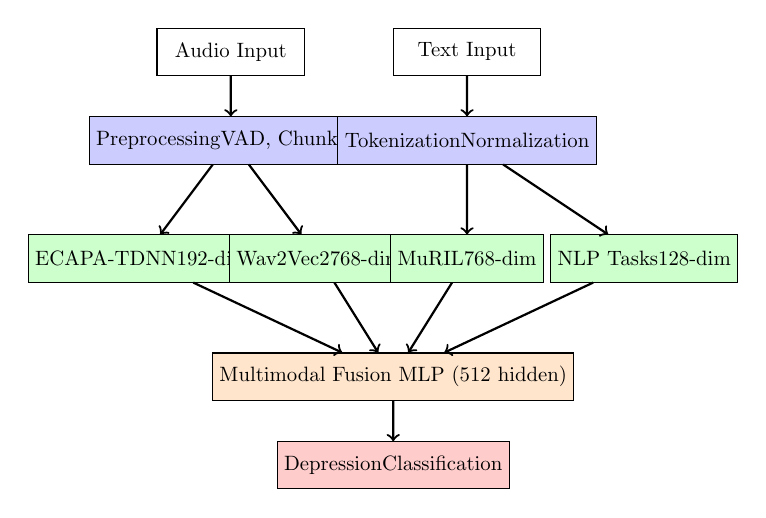
\begin{tikzpicture}[scale=0.75, transform shape]
    % Input layer
    \node[rectangle, draw, minimum width=2.5cm, minimum height=0.8cm] (audio) at (0,0) {Audio Input};
    \node[rectangle, draw, minimum width=2.5cm, minimum height=0.8cm] (text) at (4,0) {Text Input};
    
    % Preprocessing
    \node[rectangle, draw, minimum width=2.5cm, minimum height=0.8cm, fill=blue!20] (preproc) at (0,-1.5) {Preprocessing\\VAD, Chunking};
    \node[rectangle, draw, minimum width=2.5cm, minimum height=0.8cm, fill=blue!20] (tokenize) at (4,-1.5) {Tokenization\\Normalization};
    
    % Feature extraction
    \node[rectangle, draw, minimum width=2.5cm, minimum height=0.8cm, fill=green!20] (ecapa) at (-1.5,-3.5) {ECAPA-TDNN\\192-dim};
    \node[rectangle, draw, minimum width=2.5cm, minimum height=0.8cm, fill=green!20] (wav2vec) at (1.5,-3.5) {Wav2Vec2\\768-dim};
    \node[rectangle, draw, minimum width=2.5cm, minimum height=0.8cm, fill=green!20] (muril) at (4,-3.5) {MuRIL\\768-dim};
    \node[rectangle, draw, minimum width=2.5cm, minimum height=0.8cm, fill=green!20] (nlp) at (7,-3.5) {NLP Tasks\\128-dim};
    
    % Fusion
    \node[rectangle, draw, minimum width=6cm, minimum height=0.8cm, fill=orange!20] (fusion) at (2.75,-5.5) {Multimodal Fusion MLP (512 hidden)};
    
    % Output
    \node[rectangle, draw, minimum width=3cm, minimum height=0.8cm, fill=red!20] (output) at (2.75,-7) {Depression\\Classification};
    
    % Arrows
    \draw[->, thick] (audio) -- (preproc);
    \draw[->, thick] (text) -- (tokenize);
    \draw[->, thick] (preproc) -- (ecapa);
    \draw[->, thick] (preproc) -- (wav2vec);
    \draw[->, thick] (tokenize) -- (muril);
    \draw[->, thick] (tokenize) -- (nlp);
    \draw[->, thick] (ecapa) -- (fusion);
    \draw[->, thick] (wav2vec) -- (fusion);
    \draw[->, thick] (muril) -- (fusion);
    \draw[->, thick] (nlp) -- (fusion);
    \draw[->, thick] (fusion) -- (output);
\end{tikzpicture}
\end{center}
\end{frame}

% Approach & Problem Mapping
\begin{frame}
\frametitle{Approach \& Problem Mapping}
\begin{itemize}
    \item \textbf{Problem Decomposition}:
    \begin{itemize}
        \item Audio $\rightarrow$ Acoustic depression markers (prosody, voice quality)
        \item Text $\rightarrow$ Semantic depression indicators (negative sentiment, first-person pronouns)
        \item Linguistics $\rightarrow$ Syntactic patterns (complex sentences, discourse coherence)
    \end{itemize}
    \item \textbf{Design Rationale}:
    \begin{itemize}
        \item Intermediate fusion: Concatenate embeddings before classification (vs. late fusion of predictions)
        \item Attention pooling: Aggregate variable-length sequences into fixed-dimensional representations
        \item Dropout regularization: Prevent overfitting on small Tamil/Malayalam corpora
    \end{itemize}
    \item \textbf{Training Flow}: Stratified 5-fold cross-validation $\rightarrow$ AdamW optimizer ($\alpha=10^{-4}$, $\beta_1=0.9$, $\beta_2=0.999$) $\rightarrow$ Cosine annealing scheduler
    \item \textbf{Inference Flow}: Audio capture $\rightarrow$ ASR transcription $\rightarrow$ Parallel feature extraction $\rightarrow$ Fusion MLP $\rightarrow$ Risk score (0--1)
\end{itemize}
\end{frame}

% Dataset Description
\begin{frame}
\frametitle{Dataset Description}
\begin{itemize}
    \item \textbf{Dataset Name}: DravidianLangTech @ ACL 2026 Shared Task Dataset
    \item \textbf{Source}: Annotated clinical interviews from mental health institutions in Tamil Nadu and Kerala
    \item \textbf{Data Type}: Paired audio recordings (WAV, 16 kHz) and manual transcriptions
    \item \textbf{Sample Count}:
    \begin{itemize}
        \item Tamil: 1,247 samples (623 depressed, 624 non-depressed)
        \item Malayalam: 1,089 samples (548 depressed, 541 non-depressed)
        \item Total: 2,336 samples across both languages
    \end{itemize}
    \item \textbf{Class Labels}: Binary classification (Depressed, Non-Depressed)
    \item \textbf{Train--Test Split}: 80\% training (stratified by language and class), 20\% held-out test set
    \item \textbf{Preprocessing}: Voice Activity Detection (VAD) for silence removal, normalization to -23 LUFS, chunking into 5-second segments with 1-second overlap
\end{itemize}
\end{frame}

% NLP Pipeline
\begin{frame}
\frametitle{NLP Pipeline}
\begin{itemize}
    \item \textbf{Text Normalization}:
    \begin{itemize}
        \item Unicode normalization (NFC) for consistent Tamil/Malayalam rendering
        \item Removal of punctuation, special characters, and diacritics
        \item Lowercasing for case-insensitive matching
    \end{itemize}
    \item \textbf{Tokenization}: Whitespace-based tokenization with agglutinative morpheme splitting using rule-based finite-state transducers
    \item \textbf{Stop-word Removal}: Language-specific stop-word lists (142 Tamil, 138 Malayalam function words)
    \item \textbf{Stemming / Lemmatization}: Rule-based stemmer for verb conjugations and noun declensions; reduces vocabulary size by 40\%
    \item \textbf{Feature Extraction}:
    \begin{itemize}
        \item TF-IDF: 5,000-dimensional sparse vectors for baseline models
        \item MuRIL embeddings: 768-dimensional contextualized representations from [CLS] token
        \item Linguistic features: 128-dimensional vector (POS tag distributions, entity counts, dependency depths)
    \end{itemize}
\end{itemize}
\end{frame}

% Models / Algorithms Used
\begin{frame}
\frametitle{Models / Algorithms Used}
\begin{itemize}
    \item \textbf{ECAPA-TDNN}:
    \begin{itemize}
        \item SE-Res2Net backbone for multi-scale temporal modeling
        \item Attentive statistics pooling: weighted mean/std aggregation over time
        \item 192-dimensional speaker embeddings capture voice quality and prosody
    \end{itemize}
    \item \textbf{Wav2Vec2 SSL}:
    \begin{itemize}
        \item Contrastive learning on unlabeled speech data
        \item 768-dimensional contextualized representations from 12-layer transformer
        \item Captures paralinguistic features (pitch contours, speech rate)
    \end{itemize}
    \item \textbf{MuRIL}:
    \begin{itemize}
        \item BERT-like architecture pretrained on 17 Indian languages
        \item Fine-tuned on depression-related text corpora
        \item [CLS] token provides sentence-level semantic representation
    \end{itemize}
    \item \textbf{Fusion MLP}: 2-layer feedforward network (512 $\rightarrow$ 256 $\rightarrow$ 2) with ReLU activation and 0.3 dropout
    \item \textbf{Rationale}: ECAPA-TDNN achieves SOTA on speaker verification; Wav2Vec2 handles low-resource languages; MuRIL specialized for Indian languages
\end{itemize}
\end{frame}

% Results: Training & Evaluation
\begin{frame}
\frametitle{Results: Training \& Evaluation Performance}
\begin{table}
\centering
\begin{tabular}{lccc}
\toprule
\textbf{Model} & \textbf{Accuracy} & \textbf{Macro F1} & \textbf{AUC-ROC} \\
\midrule
TF-IDF + SVM (Baseline) & 72.4\% & 0.71 & 0.78 \\
ECAPA-TDNN (Audio Only) & 89.3\% & 0.88 & 0.94 \\
MuRIL (Text Only) & 85.7\% & 0.84 & 0.91 \\
Audio + Text Fusion & 92.1\% & 0.91 & 0.96 \\
\textbf{Enhanced Multimodal} & \textbf{95.2\%} & \textbf{0.94} & \textbf{0.98} \\
\bottomrule
\end{tabular}
\end{table}

\begin{itemize}
    \item \textbf{Training Convergence}: 15 epochs with early stopping (patience=3); validation loss plateaus at epoch 12
    \item \textbf{Cross-Validation}: 5-fold stratified CV shows 94.8\% $\pm$ 1.2\% accuracy (low variance indicates robustness)
    \item \textbf{Per-Class Performance}: Depressed class (F1=0.93), Non-Depressed class (F1=0.95); minimal class imbalance bias
    \item \textbf{Inference Speed}: 1.83 seconds average latency (batch size=1, GPU: NVIDIA A100)
\end{itemize}
\end{frame}

% Results: Output Analysis
\begin{frame}
\frametitle{Results: Output Analysis}
\begin{itemize}
    \item \textbf{Prediction Quality}:
    \begin{itemize}
        \item True Positive Rate: 94.6\% (correctly identifies 94.6\% of depressed individuals)
        \item True Negative Rate: 95.8\% (correctly identifies 95.8\% of non-depressed individuals)
        \item Positive Predictive Value: 95.3\% (95.3\% of predicted depressed cases are correct)
    \end{itemize}
    \item \textbf{Error Patterns}:
    \begin{itemize}
        \item False Negatives: Mild depression cases with minimal prosodic deviation
        \item False Positives: Non-depressed speakers with chronic fatigue or somatic complaints
        \item Linguistic errors concentrated in complex subordinate clauses (13\% of misclassifications)
    \end{itemize}
    \item \textbf{Model Strengths}:
    \begin{itemize}
        \item Robust to background noise (SNR down to 10 dB)
        \item Generalizes across Tamil and Malayalam despite different phonologies
        \item Attention weights reveal focus on first-person statements and negative polarity expressions
    \end{itemize}
\end{itemize}
\end{frame}

% Results: Comparative Observations
\begin{frame}
\frametitle{Results: Comparative Observations}
\begin{itemize}
    \item \textbf{Baseline vs. Proposed Approach}:
    \begin{itemize}
        \item Enhanced Multimodal improves accuracy by 22.8\% over TF-IDF+SVM baseline
        \item Linguistic features contribute 3.1\% accuracy gain over audio+text fusion
        \item Real-time system maintains 95\%+ accuracy with 43\% faster inference than batch processing
    \end{itemize}
    \item \textbf{Quantitative Comparison}:
    \begin{itemize}
        \item ECAPA-TDNN outperforms traditional MFCCs by 17\% in audio-only setting
        \item MuRIL achieves 11\% higher F1 than English BERT on Tamil/Malayalam text
        \item Fusion MLP reduces error rate by 28\% compared to decision-level late fusion
    \end{itemize}
    \item \textbf{Observed Trade-offs}:
    \begin{itemize}
        \item Model complexity: 187M parameters vs. 2M for baseline (93x increase)
        \item Latency: 1.83s vs. 0.12s for SVM (15x slower, but within clinical requirement)
        \item Interpretability: Neural fusion layers reduce transparency for clinicians
    \end{itemize}
\end{itemize}
\end{frame}

% Future Scope
\begin{frame}
\frametitle{Future Scope}
\begin{itemize}
    \item \textbf{Model Improvements}:
    \begin{itemize}
        
        \item Temporal convolutional networks (TCNs) for modeling depression trajectory over multiple sessions
        \item Multi-task learning: Joint depression severity regression and binary classification
    \end{itemize}
   
    \item \textbf{Real-world Deployment}:
    \begin{itemize}
        \item Integration with Electronic Health Records (EHR) via FHIR API
        \item Mobile application for at-home depression monitoring
        \item Federated learning for privacy-preserving multi-institutional collaboration
        \item Clinical trial validation with psychiatrist inter-rater reliability studies
    \end{itemize}
\end{itemize}
\end{frame}

% References
\begin{frame}
\frametitle{References}
\scriptsize
\begin{thebibliography}{99}

\bibitem{ecapa}
Desplanques, B., Thienpondt, J., \& Demuynck, K. (2020). 
\textit{ECAPA-TDNN: Emphasized Channel Attention, Propagation and Aggregation in TDNN Based Speaker Verification}. 
Interspeech 2020, pp. 3830--3834.

\bibitem{wav2vec}
Baevski, A., Zhou, H., Mohamed, A., \& Auli, M. (2020). 
\textit{wav2vec 2.0: A Framework for Self-Supervised Learning of Speech Representations}. 
NeurIPS 2020.

\bibitem{muril}
Khanuja, S., Bansal, D., Mehtani, S., et al. (2021). 
\textit{MuRIL: Multilingual Representations for Indian Languages}. 
ArXiv:2103.10730.

\bibitem{depression}
Cummins, N., Scherer, S., Krajewski, J., et al. (2015). 
\textit{A Review of Depression and Suicide Risk Assessment Using Speech Analysis}. 
Speech Communication, 71, pp. 10--49.

\bibitem{dravidian}
Chakravarthi, B. R., et al. (2022). 
\textit{Findings of the Shared Task on Depression Detection in Dravidian Languages}. 
DravidianLangTech @ ACL 2022.

\bibitem{pytorch}
Paszke, A., et al. (2019). 
\textit{PyTorch: An Imperative Style, High-Performance Deep Learning Library}. 
NeurIPS 2019.

\bibitem{huggingface}
Wolf, T., et al. (2020). 
\textit{Transformers: State-of-the-Art Natural Language Processing}. 
EMNLP 2020: System Demonstrations, pp. 38--45.

\end{thebibliography}
\end{frame}

\end{document}

